
\chapter{Appendix-2}\label{Appendix-2}
\section{Deep Neural Networks}\label{SI:neuralnets}
Broadly, neurons are the fundamental processing elements of a neural network.
They receive their inputs $(x_{ij})$ as the weighted $(w_{ij})$ outputs from the neurons in the previous layers and produce a single output signal $(y_j)$ dependent upon a bias $(b_j)$ and activation function $f(*)$

\begin{equation}
      z_j = \sum_i^n w_{ij}  x_{ij}+b_j
\end{equation}
\begin{equation}
    y_j = f(z_j)
\end{equation}

More specifically, “Deep” neural networks are a collection of such neurons organized as distinct layers.
A neural network approximates a function by fine tuning its weights and biases so that its output signal closely resembles the output of the function it is approximating for the same inputs.
The degree of resemblance between the signals is computed based on a loss function $L(*)$

\begin{equation}
    Loss = L(Q_p,Q_o)
\end{equation}
\begin{equation}
    w_{ij} = w_{ij}- \alpha \times  \frac{dL(Q_p,Q_o )}{(dw_{ij})}
\end{equation}
\begin{equation}
    b_j = b_j- \alpha \times  \frac{dL(Q_p,Q_o )}{(db_j)}
\end{equation}
The choice of the loss function is dictated by the nature of the function being approximated.
For example, a neural network approximating rainfall runoff may use mean squared error\cite{tokar1999rainfall}

\begin{equation}
    Loss = |Q_p-Q_o|^2
\end{equation}
The closer the correspondence between the signals, lower the loss.

\

Neural networks minimize the loss though stochastic gradient descent, starting with a set of weights and biases (either random or values sampled from a distribution).
Based on the value of loss function, the values of weights and biases are adjusted, and the neural network attempts to approximate the function with these updated values.
This process of tuning the weights and biases is repeated until the neural network can approximate the function to satisfaction or loss is minimized.
While Deep Neural Networks show significant promise in approximating functions, their ability to do so is contingent upon several factors: Stability of the learning process, the size and depth of the network, the underlying data distributions~\cite{goodfellow2016Deep,chollet2017Deep}.
Fundamental description of Deep Neural Networks can be found in established textbooks~\cite{goodfellow2016Deep}.

\section{Hyper parameters and architecture}\label{SI:hyperparams}

\noindent\textbf{Neural Network}
\begin{table}[H]
\begin{tabular}{ll}
\toprule
Layers                      & 2  \\
Number of Neurons per layer & 50 \\
\bottomrule
\end{tabular}
\end{table}

\noindent\textbf{Gradient Descent}
\begin{table}[H]
\begin{tabular}{ll}
\toprule
Learning Rate                      & $10^{-3}$  \\
Rho & 0.9 \\
Epsilon & $10^{-8}$ \\
Decay & 0.0\\
\bottomrule
\end{tabular}
\end{table}

\noindent\textbf{Batch Normalization}
\begin{table}[H]
\begin{tabular}{ll}
\toprule
Momentum                     & 0.99  \\
Epsilon & 0.001 \\
\bottomrule
\end{tabular}
\end{table}

\noindent\textbf{Deep Q Network}
\begin{table}[H]
\begin{tabular}{ll}
\toprule
Target Network Update                     & 10000  \\
Gamma & 0.99\\
Replay Buffer & 100000 \\
\bottomrule
\end{tabular}
\end{table}


\section{Equal-filling degree algorithm}\label{SI:equalfill}

\begin{figure}[H]
	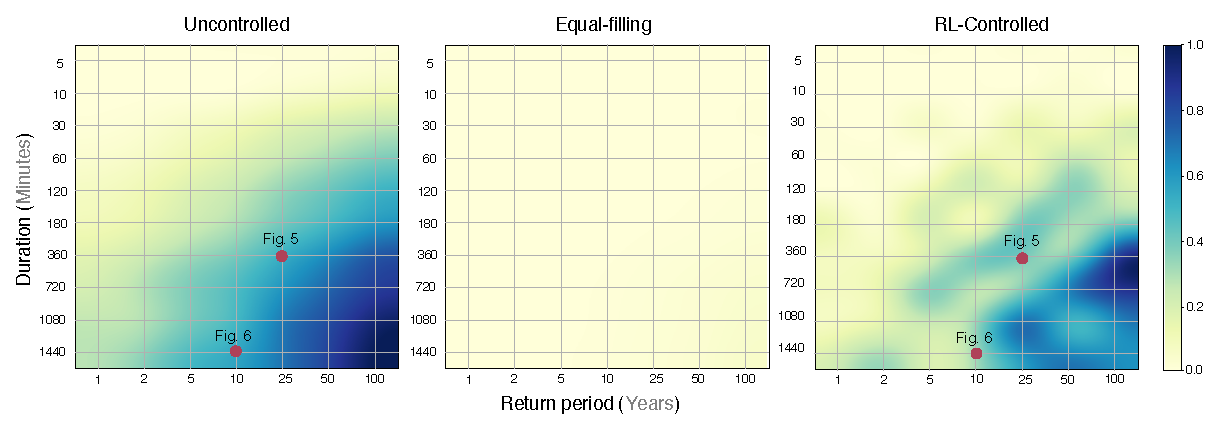
\includegraphics[width=\linewidth]{gfx/Chapter-3/heatmap_eq.eps}
	\caption{Performance comparison between uncontrolled and controlled systems (RL and equal-filling) across a spectrum of stormevents. Equal-filling approach is able to successfully control the system to achieve the objective of minimizing flows in all the stormevents.}\label{fig:11}
\end{figure}


Equal filling degree algorithm is a rule based real-time control approach for controlling stormwater networks.
In this approach, control decisions of either releasing or holding back water, are made based on the filling degree (${f}_i$) in the controlled asset ($i$).
In this context, filling degree is defined as the normalized depth in an asset.
By releasing water based on the difference between the average filling degree of the network ($\bar{f}$) and the filling degree (${f}_i$) in each asset, equal-filling approach ensures that the storage potential in the control assets is utilized uniformly.  

\begin{algorithm}
	\caption{Equal-Filling Control Algorithm: Let $i$ be a basin in the network of $\mathcal{N}$ tanks. In this scenario, $\mathcal{N} = 4$.}\label{efd}
\For{all $\mathcal{N}$ tanks}{Compute the \textit{filling degree}; $f^i = \frac{\text{depth}^i}{\text{Max depth}^i}$}
Estimate the \textit{average filling degree}; $\bar{f} = \frac{\sum^N_i f^i}{N}$\\
\For{all $\mathcal{N}$ tanks}{\If{$f^i > \bar{f}$}{$valve^i = c \times (f^i - \bar{f})$}
	\ElseIf{$\bar{f} - f^i \leq \theta$}{$valve^i = \bar{f}$}
	\Else{$valve^i = 0.0$}

}
\end{algorithm}

Hyper-parameter $c$ can be used to regulate the valve opening and $\theta$ can be used to control the flashiness of the outflow hydrograph.
In this study, these parameters were chosen to be 3.0 and 0.18 respectively.
Performance of the equal-filling algorithm across the 70 rainevents is presented in figure~\ref{fig:11}.
Performance of the equal-filling control approach in controlling a 6 hour 25 year is presented in figure~\ref{fig:12}.

\begin{figure}[H]
    \centering
    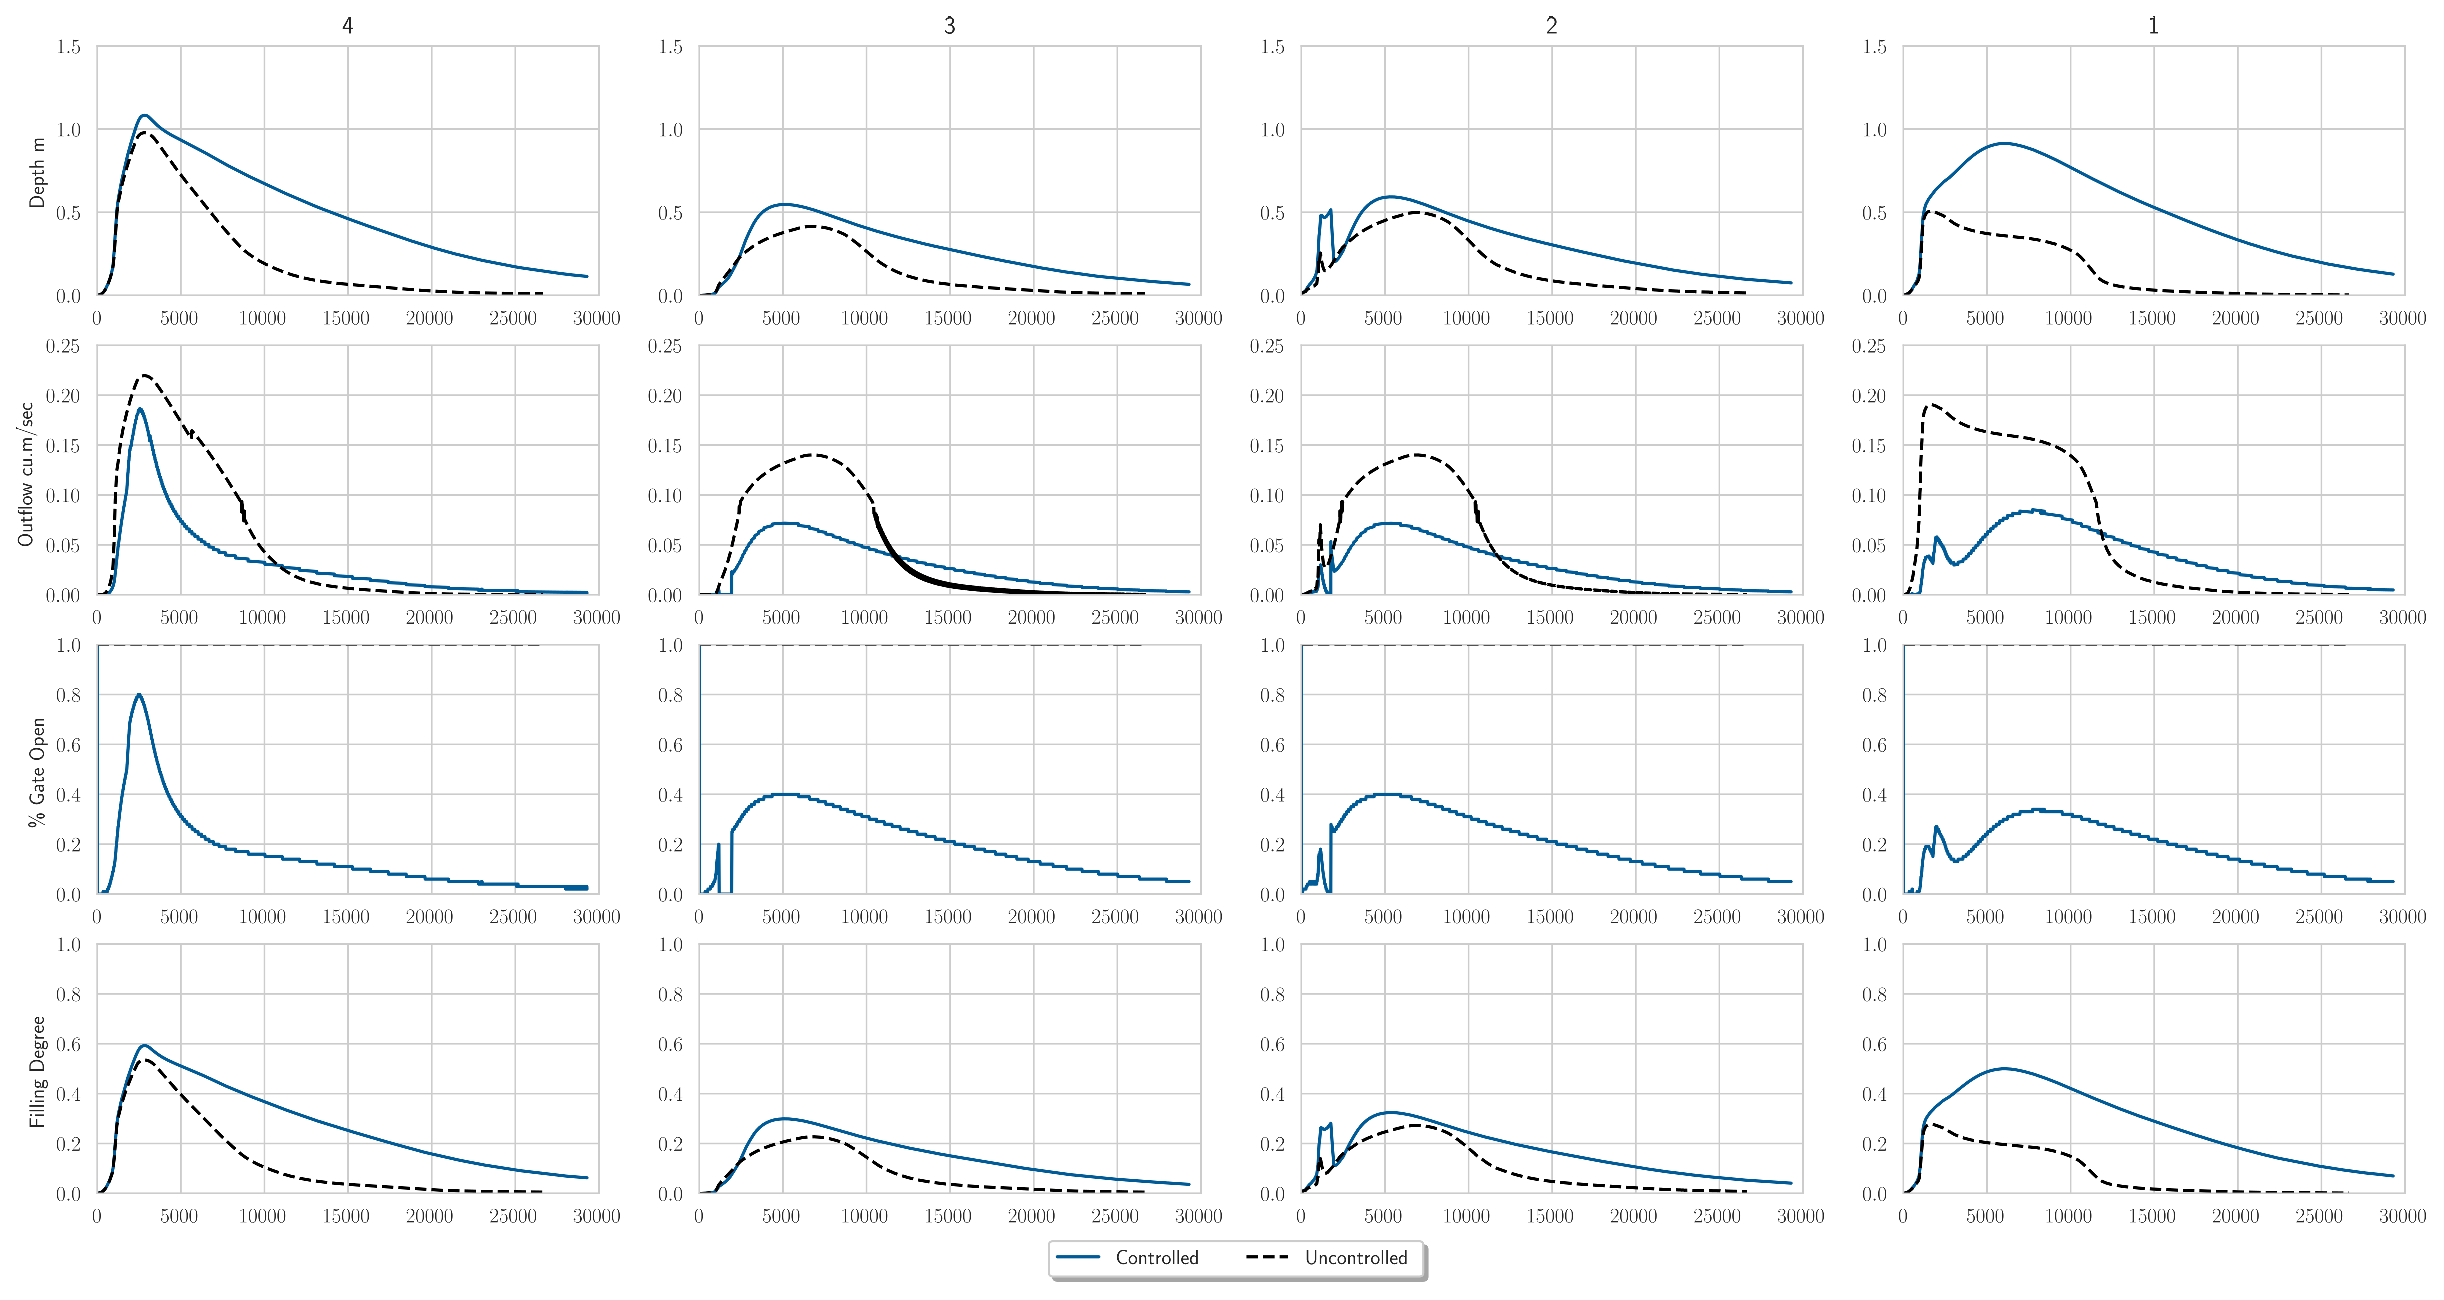
\includegraphics[width=\linewidth]{gfx/Chapter-3/eqf.eps}
    \caption{Equal-filling approach successfully maintains the outflows from the four basins below the desired threshold.}\label{fig:12}
\end{figure}

\section{Scenario 1 --- Reward function Formulation Sensitivity}\label{SI:reward-math}

\noindent Reward functions 3a and 3b are formulated as a variant of the third reward function (eq.11) to analyse the sensitivity of the agent's performance to the choice of equation used in the formulation reward functions.
Reward function 3a (eq.~\ref{third1}) is formulated using exponential and the 3b reward function is built using squared terms (eq.~\ref{third2}).

\begin{equation}
  r_{3a} (s_t) = \left\{ \begin{array}{ll}
    c_1 - c_2 e^{h_t}, & h_t < Hf_t \leq F\\
    c_1 - c_3 e^{h_t}, & h_t \geq Hf_t \leq F\\
    - e^{f_t} - c_2 e^{h_t} + c_4, & h_t < Hf_t > F\\
    - e^{f_t} - c_3 e^{h_t} + c_4, & h_t \geq Hf_t > F
  \end{array} \right.\label{third1}
\end{equation}

\begin{align}
  r_{3b} (s_t) = \left\{ \begin{array}{ll}
    c_1 - c_2 h_t^2, & h_t < Hf_t \leq F\\
    c_3 - c_4 h_t^2, & h_t \geq Hf_t \leq F\\
    - c_5 {(c_6 f_t)}^2 - c_2 h_t^2 + c_7, & h_t < Hf_t > F\\
    - c_5 {(c_6 f_t)}^2 - c_4 h_t^2 + c_7, & h_t \geq Hf_t > F
  \end{array} \right.\label{third2}
\end{align}

3a and 3b reward function are parametrized by $\{ c_1 = 2.5, c_2 = 0.5, c_3 = 0.75, c_4=3\}$ and $\{c_1 =2.0, c_2 = 0.5, c_3 = 2.5, c_4 = 0.9, c_5=0.1, c_6=10, c_7 = 1.5\}$ respectively.
These parameters are chosen to constrain the scale of these reward functions to the third reward function.

\begin{figure}[H]
    \centering
    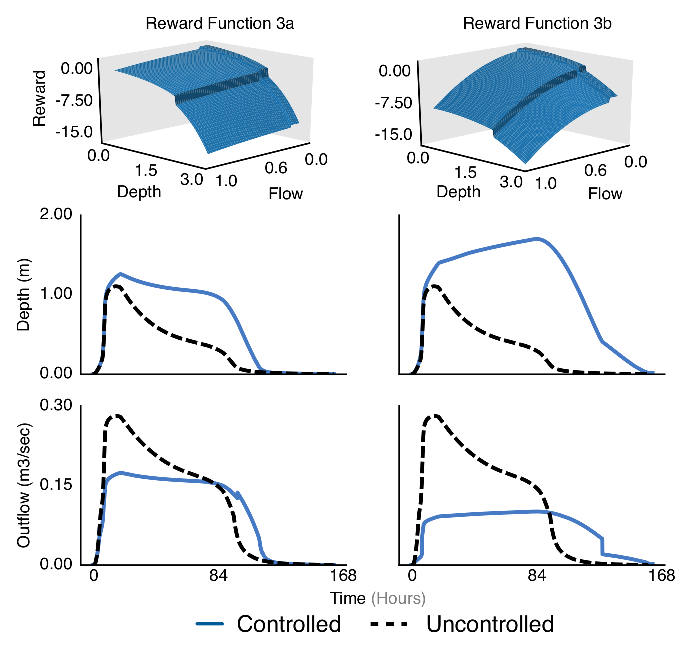
\includegraphics[width=0.6\linewidth]{gfx/Chapter-3/new_reward.eps}
    \caption{Performance of the RL agent is independent of the choice of equations used for creating the reward functions.}\label{fig:new_reward_math}
\end{figure}

\newpage 

\section{Scenario 1 --- Location sensitivity}\label{SI:reward-loc}
\begin{figure}[H]
    \centering
    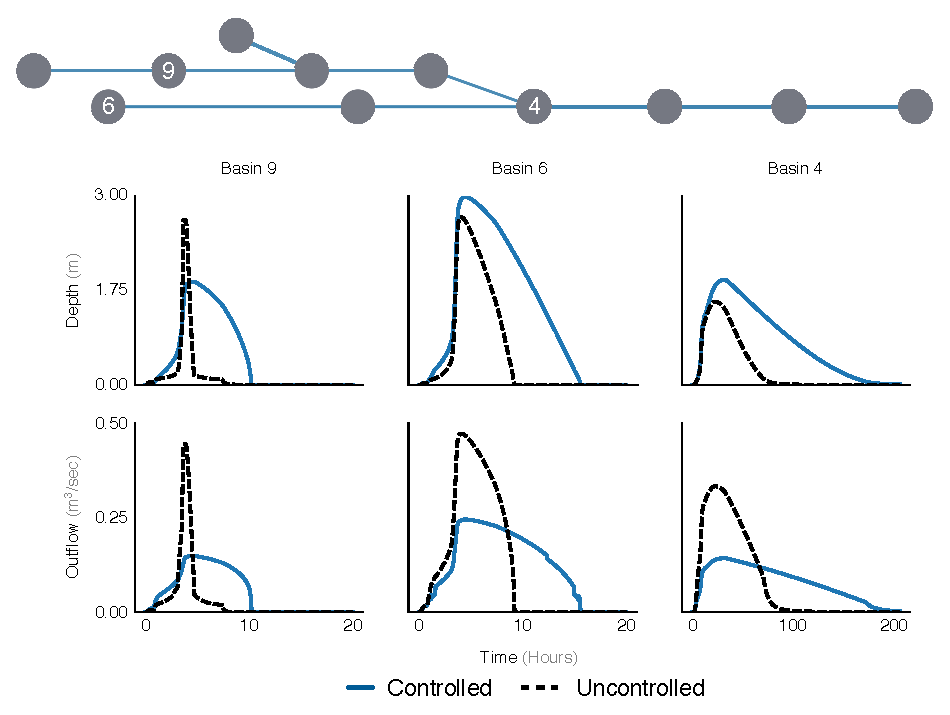
\includegraphics[width=\linewidth]{gfx/Chapter-3/location_senstiv.eps}
    \caption{Performance of the RL agent controlling the basins across the network. Controller is able to control the response of the basins irrespective of the location, indicating the independence of the control algorithm's performance on the location of the basin. Results presented in this figure are independent simulations; each column represents a simulation where only that particular basin is controlled.}\label{fig:9}
\end{figure}

\section{Scenario 2 --- Back-to-back event}\label{SI:b2b-events}

\begin{figure}[H]
    \centering
    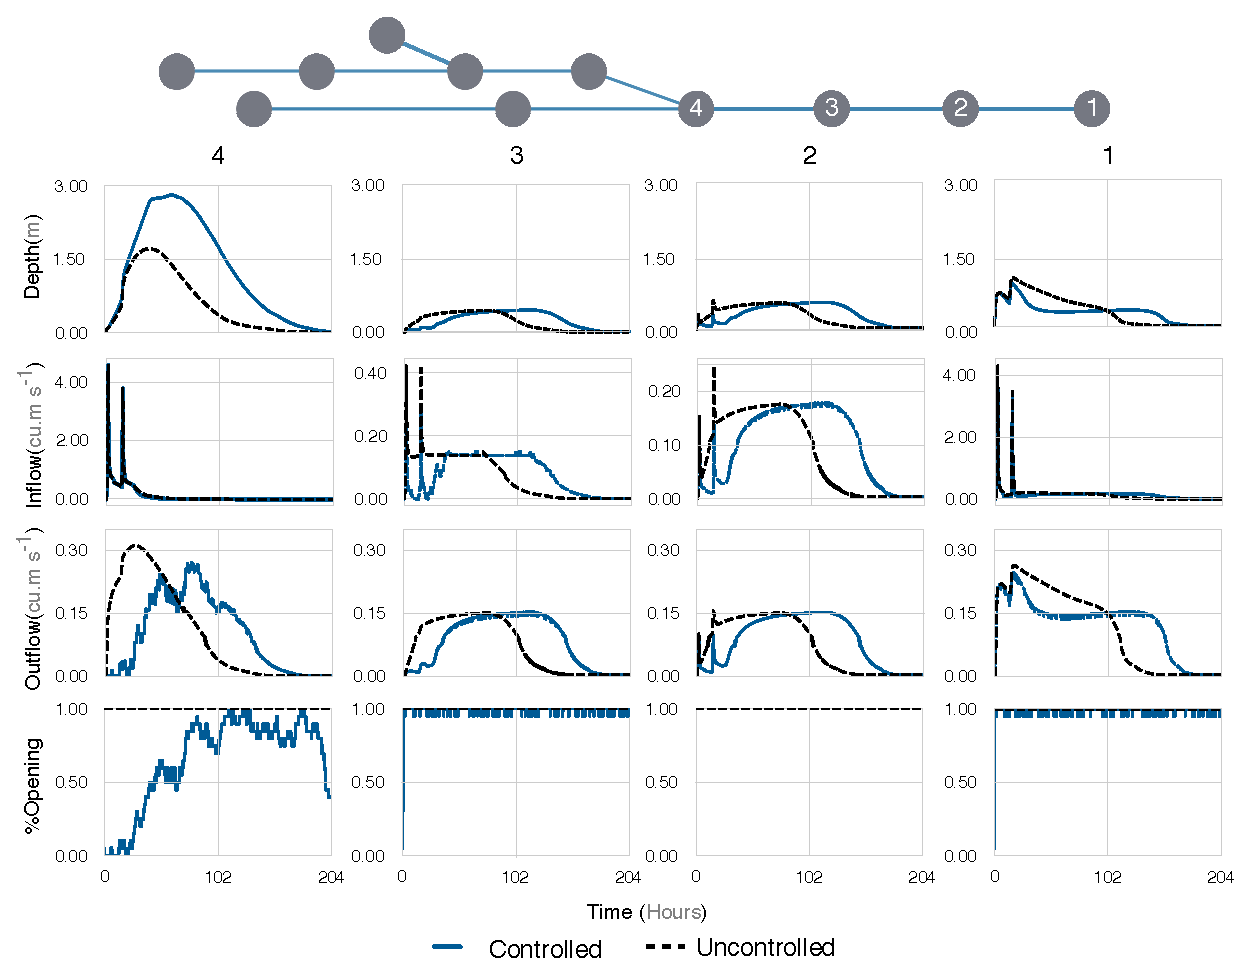
\includegraphics[width=\linewidth]{gfx/Chapter-3/b2b.eps}
    \caption{Performance of the RL controller in a back-to-back event. Given that the controller is trained to react based on the depth in the basins and not the rainfall experienced in the watershed, controller treats this back-to-back event as if it were a single event.}\label{fig:10}
\end{figure}

